\documentclass[UTF8]{ctexart}
\usepackage{mathtools,wallpaper}
\usepackage{t1enc}
\usepackage{pagecolor}
\usepackage{enumitem}
\usepackage{hyperref}
\usepackage{graphicx}
\usepackage{listings}
\usepackage{amssymb}
\usepackage[dvipsnames]{xcolor}
\usepackage{float}
\usepackage{numerica}


\begin{document}

\section{Undecidability}
\subsection{The Church-Turing thesis丘奇图灵定理}

丘奇图灵理论中，算法 是 一个在所有输入上都可以停机并且能够判定语言并且可计算的图灵机。不能被图灵机执行的计算任务是无法实现并且undecidable。

这一章研究通用图灵机，针对我们之前的串行图灵机，虽然也和这个有点相似，但是之前的串行图灵机主要研究固定任务的简单衔接，而本章我们希望通过先定义图灵机的统一编码规则（也就是用同一台图灵机的某个语言对某个问题进行描述并且放入此通用图灵机能够直接运行），来实现机器处理自身编码能力，而非通过问题思考如何解决此问题来设计图灵机。

\subsection{Universal Turing Machines 通用图灵机设计}

\begin{itemize}
    \item 设计通用图灵机
    \begin{enumerate}
        \item 在字母表中，我们对状态和带符号编码为字符串形式，一个表示图灵机状态的字符串形式是以q为开头后跟0到多个0或者1组成的字符串（q后跟着一个二进制字符串）；纸带上字符用a后跟二进制字符串进行表示。
        \item 我们定义一个五元组的图灵机，i满足2的i次方大于等于状态数量的最小整数，j是满足2的j次方大于等于字符表数量+2的最小整数。同时，定义空一直是$a0^j$,右三角号为$a0^{j-1}1$,左箭头为$a0{j-2}10$,右箭头为$a0{j-2}11$.起始状态为$q0^i$
        \item 我们将图灵机表示为M,[M]表示着M的状态转移表，转移表会写成四元组的形式(q,a,p,b),q表示当前状态，a表示当前指针头扫描到的字符，p表示下一个状态编码，b表示要执行的动作（包括要写的字符以及指针头移动的方向）。
        \item 起始状态(s,$\sqcup $)。停机状态H通过找到M图灵机中转移方程四元组中不作为第一个分量的状态来间接确定。如果M decides a language, H=\{y,n\}.
        \item 这样任何图灵机都能被表示。并且任何属于字符串子集的的字符串都有一个唯一的表示，denoted 为 w。
        \item eg1
        \begin{figure}[H]
            \centering
            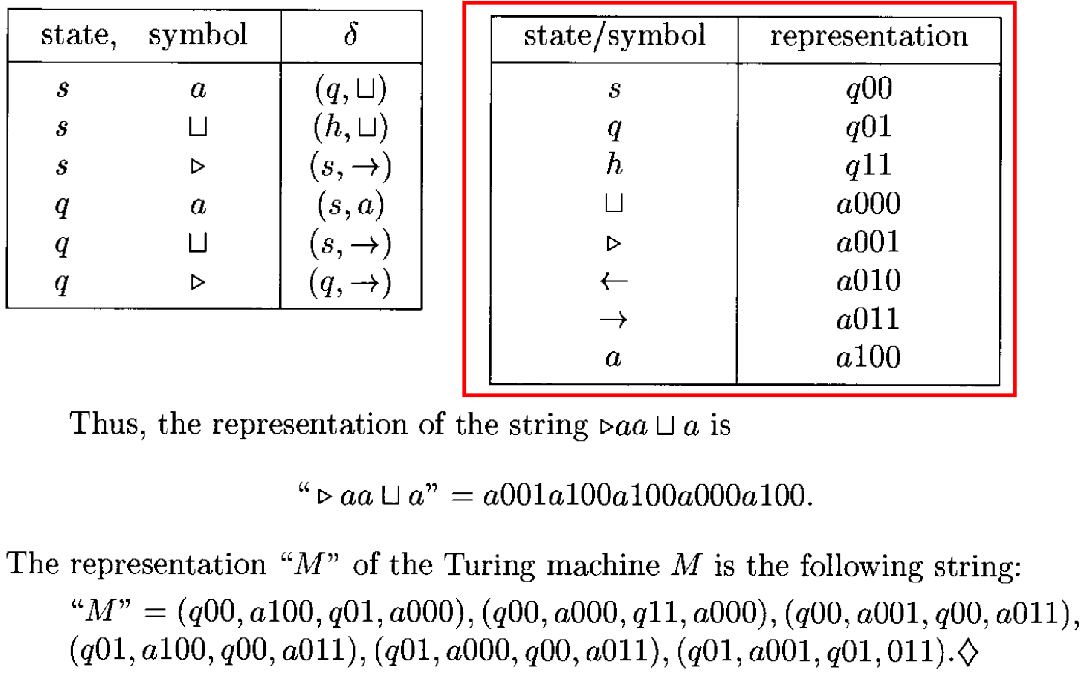
\includegraphics[width=1\textwidth]{static/UniversalTM.png}
            \caption{UniversalTM}
            \label{UniversalTM}
        \end{figure}    
    \end{enumerate}

    \item 如何使用通用图灵机，denoted U，模拟其他图灵机
    
    通用图灵机可以接受两个参数，一个是另一台图灵机M的描述"M",另一个是输入字符串w的描述。如果我们要让U模拟M的行为，我们要满足：U在M，w两个输入能够停机当且仅当M在输入w上停机。

    $U([M],[w]_{M})=[M(w)]_M$
    $[w]_{M}$表明w是针对图灵机M的字母表和编码规则进行编码。在w的编码中，我们可以使用通用图灵机对M编码的w进行转换，并且能够计算。

    \begin{enumerate}
        \item 我们先使用三带通用图灵机U‘模拟图灵机M的操作，直接使用单带图灵机对M模拟过于复杂，如果三带图灵机能够模拟出M的操作，由定理多带图灵机等价于单带图灵机，所以如果我们能够使用三带图灵机对M进行模拟，那么我们同样也能够使用单带图灵机对M进行模拟。
        \item U‘的三条带子，第一条纸带存储M当前的带内容，第二条纸带存储M的描述让U'可以查阅M的状态方程，第三条纸带存储M的当前状态编码。
        \item 首先U‘将M编码复制到U’的第二条纸带，并且将输入w的编码移动到以$\vartriangleright \sqcup $为起点的第一个纸带形成$\vartriangleright \sqcup w$,U'在第三条纸带写上M的初始状态编码。
        \item U'模拟M的操作：第一条纸带的读写头对准M当前扫描的符号所对应的编码字符串，第二条纸带和第三条纸带在两次模拟之间会停留在纸带的左端。U’扫描第二条纸带，直到找到第一个四元组，四元组的第一个分量与第三条纸带上写入的分量相匹配，第二个分量与第一条纸带上当前扫描到的符号相匹配，若找到这样的四元组，U‘将状态更新为第三个分量，并且在第一条纸带上执行第四个分量所指定的操作。若第四个分量是M带字母表中某一符号的编码，则将符号编码串写入第一条纸带；若第四条纸带是左移编码，U‘将第一条带子的读写头移至左侧第一个以a左侧第一个以a开头的符号编码处，若遇到右三角号，转换为空白符的编码。
        \item 若某一步中，状态符号组合不能满足第二条纸带中的任何四元组，那么为停机状态。
    \end{enumerate}
    
\end{itemize}

\subsection{The halting problem 停机问题}

停机问题定义：对于停机判定程序，我们使用设计一个程序（停机判定程序）的语言设计程序P以及输入X。如果一个程序判断输入X是否会在输入的程序P停机，那么我们称这个程序为halts(P,X).
$Halt_{TM}$=\{<M,w>|TM M halts on input string w\}

\begin{itemize}
    \item 如何证明存不存在停机程序能够判断所有程序能够在某个输入停机？
    
    证明1
    \begin{enumerate}
        \item 设计一个对角程序 diagonal(X):X程序以自身为输入的停机程序，如果此停机程序停机，那么不断执行此程序，如果此停机程序不停机，则停机。如果halt(X,X)=yes 那么diagonal(X)一直循环，否则diagonal(X)停机
        \item 那么证明1中我们使用对角化的思想，构造diagonal(diagonal),如果diagonal(diagonal)停机，halts(diagonal,diagonal)不停机->diagonal在diagonal上不停机，与我们假设diagonal(diagonal)矛盾。
    \end{enumerate}

    证明2
    \begin{enumerate}
        \item 定义停机问题$H$=\{<M,w>|TM M halts on input string w\}。我们知道H是递归可枚举的，因为停机问题H能够被universal turing machine 半判定，就是如果输入属于我们的程序能够判定的，那么就停机返回yes，如果不属于那么就不断循环，我们可以使用通用模型U‘来模拟H的输入输出和状态。并且如果一个停机问题能够是decidable，那么所有程序在任意某个输入都会停机，也就是说所有recursive enumerable languages都是可判定的。
        \item 我们假设H是可以被图灵机M0判定，给定一个图灵机M半判定语言L(M),我们可以设计一个图灵机M‘来判定L(M)，首先将M‘输入改为M0的输入格式“M”“w”，并且模拟M0的行为，如果M0 accept w，那么M‘ accept w；如果M0输出no，那么M‘输出no。
        \item 我们假设H1=\{"M": 图灵机M在输入为"M"上停机\}。
        \item 如果H1是递归的，那么由于闭包性它的补集也是递归的，$\overline{H1}$=\{w:w不是图灵机的编码或者w是图灵机M的编码“M”并且M在输入“M”上不停机\}。如果$M^{*}$半判定H1补集，那么图灵机$M^{*}$的编码“$M^{*}$”并且$M^{*}$在输入“$M^{*}$”上不停机，$M^{*}$不接受“$M^{*}$”。因此得出矛盾，停机问题不是可判定的，但是是半判定的。
    \end{enumerate}

    \item 定理：语言H不是递归的，因此递归语言室可枚举递归语言类的真子集（strict subset）
    
    \item 递归可枚举语言类在补运算上室不封闭的。


\end{itemize}

\subsection{Acceptance problem接受问题}

\begin{itemize}
    \item Let $A_{TM}$=\{<M,w>|M是一个图灵机并且M接受w\}
    
    $A_{TM}$ 是 undecidable但是是图灵可识别的。不可判定只是说其没有判定器，而不是说不可半判定。

    证明：
    \begin{enumerate}
        \item assume that $A_{TM}$ 是可判定问题 以及H是$A_{TM}$的判定器。对于输入(M，w)，M是图灵机，w是字符串。如果M接受w，H停机并且接受；如果M不接受w，那么H停机并且拒绝（分段函数写法）。
        \item 构建一个新的图灵机D，D=“On input <M>, where M is a TM”: 1.Run H on input <M,<M>>。2. Output the opposite of what H outputs. If H accepts, D reject and if H reject, D accept.
        \item 输入描述(D)运行D图灵机，如果D不接受<D>,那么D(<D>)接受,如果D接受<D>,那么D(<D>)拒绝。
        \item 矛盾，因此TM D和TM H不可以存在。
    \end{enumerate}

    \item $A_{TM}$是 Turing-Recognizable 图灵可识别
    
    U="On input <M,w>,where M 是一个图灵机，w是一个字符串：1.输入为w，模拟M的结果 2.如果M接受w，则接受，如果M拒绝，则拒绝，如果M循环，则循环" 

\end{itemize}

\subsection{Turing-Unrecognizable Language图灵不可识别语言}

\begin{itemize}
    \item co-Turing-recognizable：对于语言L，L的补给是图灵可识别的，我们称L为"co-Turing-recognizable"
    \item 一个语言是decidable，当且仅当此语言是图灵可识别以及co-图灵可识别。
    
    证明：

        \begin{figure}[H]
            \centering
            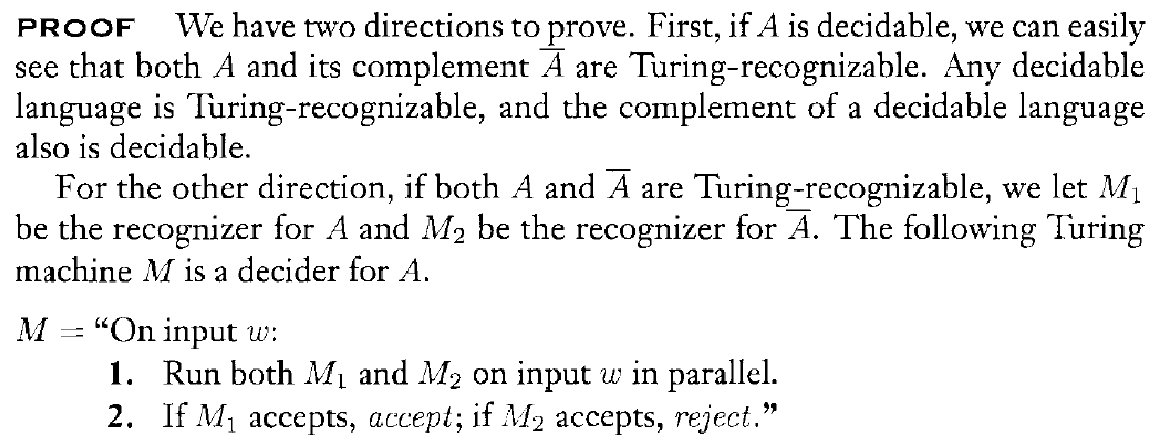
\includegraphics[width=1\textwidth]{static/Turing-recognizable-dicidable.png}
            \caption{Turing-recognizable-dicidable}
            \label{Turing-recognizable-dicidable}
        \end{figure}  

    \item 定理：$\overline{A_{TM}}$不是图灵可识别的。根据定理，$A_{TM}$ 是不可判定，并且是图灵可识别的，所以其补集为图灵不可识别的。
\end{itemize}


\end{document}